\chapter{Árboles parcialmente ordenados}
Un \textbf{árbol parcialmente ordenado} o \textbf{APO}, es un árbol completo (árbol que tiene todos sus niveles llenos menos el último que faltan nodos por la derecha) en el que el \textit{valor de cualquier nodo es menor o igual que el de todos sus descendientes}. 
\begin{figure}[h]
  \begin{center}
    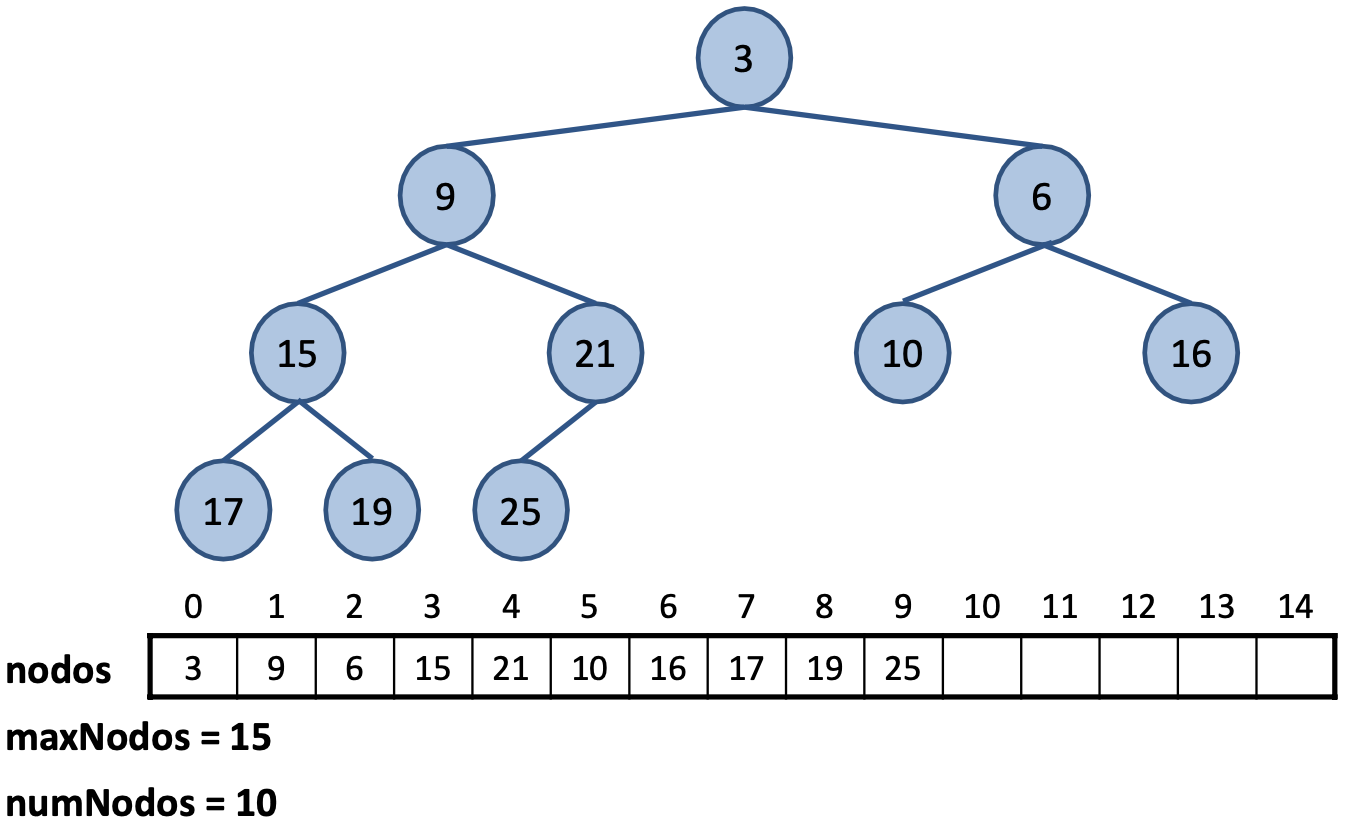
\includegraphics[width=0.7\textwidth]{assets/apo1.png}
  \end{center}
\end{figure}
\section{Operaciones básicas}
Cuando trabajamos con APOs podemos realizar varias operaciones como \textbf{acceso al mínimo valor}, \textbf{inserción} y \textbf{eliminación}.
\begin{itemize}
  \item El mínimo valor se puede obtener en un tiempo de\(O(1)\), debido a que el mínimo valor siempre será la \textbf{raíz} del propio árbol.
  \item Encontramos la \textbf{propiedad de completitud} que implica que la altura menor posible del APO de \(n\) nodos es de \(h = log_{2}\ n\).
  \item También existe la \textbf{propiedad de orden} del APO que permite efectuar inserciones y eliminaciones en el mismo en un tiempo \(O(h)\) (en el peor caso), y en un tiempo \(O(log_{2}\ n)\) en el mejor y caso promedio.
\end{itemize}

\section{Especificación del TAD árbol parcialmente ordenado}
En los árboles parcialmente ordenados vamos a encontrar dos métodos \texttt{hundir()} y \texttt{flotar()}.

\subsection*{Constructor del árbol parcialmente ordenado}
\underbar{\textit{Precondición:}} maxNodos $>$ 0\\
\underbar{\textit{Postcondición:}} Crea y devuelve un APO de tamaño MaxNodos vacío.\\
\verb|  Apo(size_t maxNodos);|

\subsection*{Inserción de elementos en el APO}
\underbar{\textit{Precondición:}} APO no lleno.\\
\underbar{\textit{Postcondición:}} Inserta el elemento en su posición correcta.\\
\verb|  void insertar(const T& e);|
\subsection*{Eliminación de elementos en el APO}
\underbar{\textit{Precondición:}} APO no vacío.\\
\underbar{\textit{Postcondición:}} Elimina la raíz reordenando el APO.
\verb|  void suprimir();|
\subsection*{Métodos observadores de un APO}
\begin{itemize}
  \item \underbar{\large\textbf{Obtener la raíz}}:\\
  \underbar{\textit{Precondición:}} APO no vacío.\\
  \underbar{\textit{Postcondición:}} Devuelve el elemento que está en la raíz.\\
  \verb|  const T& cima()const;|
  \item \underbar{\large\textbf{Obtener estado del árbol}}:\\
  \underbar{\textit{Postcondición:}} Devuelve \texttt{True} si el árbol está vacío, si no, \texttt{False}.
  \verb|  bool vacio()const;|
  \item \underbar{\large\textbf{Obtener el padre}}:\\
  \underbar{\textit{Precondición:}} APO no vacío.\\
  \underbar{\textit{Postcondición:}} Devuelve el padre del nodo n.\\
  \verb|nodo padre(nodo n)const;|
  \item \underbar{\large\textbf{Obtener el hijo izquierdo}}:\\
  \underbar{\textit{Precondición:}} APO no vacío.\\
  \underbar{\textit{Postcondición:}} Devuelve el hijo izquierdo del nodo \(n\).\\
  \verb|nodo hIzq(nodo n)const;|
  \item \underbar{\large\textbf{Obtener el hijo derecho}}:\\
  \underbar{\textit{Precondición:}} APO no vacío.\\
  \underbar{\textit{Postcondición:}} Devuelve el hijo derecho del nodo \(n\).\\
  \verb|  nodo hDer(nodo n)const;|
\end{itemize}


\subsection*{Métodos hundir y flotar de un APO}
\begin{itemize}
  \item \underbar{\large\textbf{Hundir un nodo}}:\\
  Este método irá de la mano a la hora de eliminar el nodo raíz, reordenando el árbol hasta que dicho nodo sea una hoja y lo podamos eliminar.

  Podemos tener 3 casos a la hora de eliminar la raíz del APO:
  \begin{itemize}
    \item \textbf{Caso 1: Un nodo} → Al tener un solo nodo (raíz), si la eliminamos el árbol quedará \textbf{vacío}.
    \item \textbf{Caso 2: Dos nodo} → Ahora tenemos tanto la raíz como su hijo izquierdo, por tanto, si eliminamos la raíz, su hijo izquierdo pasará a ser la nueva raíz del APO.
    \item \textbf{Caso 3: Más de dos nodo} → Si queremos eliminar una raíz que tiene más de dos nodos, el último nodo insertado será el que ocupe la posición del raíz y luego hundimos dicho nodo para poder cumplir la propiedad de orden.
  \end{itemize}
  \verb|  void hundir(nodo n);|
  \item \underbar{\large\textbf{Flotar un nodo}}:\\
  A la hora de insertar un nodo, éste se añade a la última posición del vector y luego para que se cumpla la propiedad de orden tenemos que ir `subiendo' dicho nodo hasta que encuentre su sitio.

  \verb|  void flotar(nodo n);|
\end{itemize}
\section{Implementación del TAD árbol parcialmente ordenado}
Vamos a hacer uso de la implementación mediante un \textbf{vector de posiciones relativas} ya que estos son muy útiles y eficientes cuando trabajamos con árboles completos.

La parte privada del TAD quedaría:
\begin{minted}[breaklines]{C++}
template <typename T> class Apo{
  public:
    //Métodos vistos en la Especificación del TAD.
  private:
    typedef size_t nodo; //Indice del vector.
    size_t maxNodos; //Tamaño del vector (árbol).
    size_t numNodos; //Número de nodos (último nodo del árbol)
    T* nodos; //Vector de nodos
    //Métodos privados de la clase
    nodo padre(nodo n)const;
    nodo hIzq(nodo n)const;
    nodo hDer(nodo n)const;
    void hundir(nodo n);
    void floar(nodo n);
};
\end{minted}
\newpage
\subsection*{Inserción de elementos en un APO}
\begin{figure}[h]
  \begin{center}
    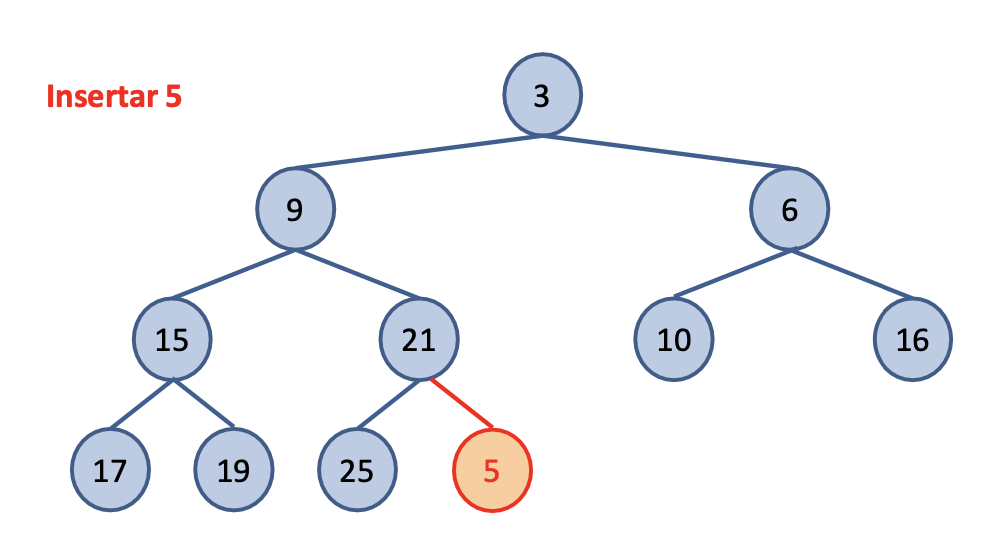
\includegraphics[width=0.7\textwidth]{assets/apo2.png}
  \end{center}
  \caption{Ejemplo de inserción 1.}
\end{figure}
Queremos insertar el valor `5' en nuestro APO el cual no está vacío, por tanto, vamos a insertarlo en la última posición del vector de posiciones relativas que equivale al hijo derecho del nodo con valor `21'. A continuación vamos flotando dicho nodo hasta que se cumpla la propiedad de ordenación.
\begin{figure}[h]
  \begin{center}
    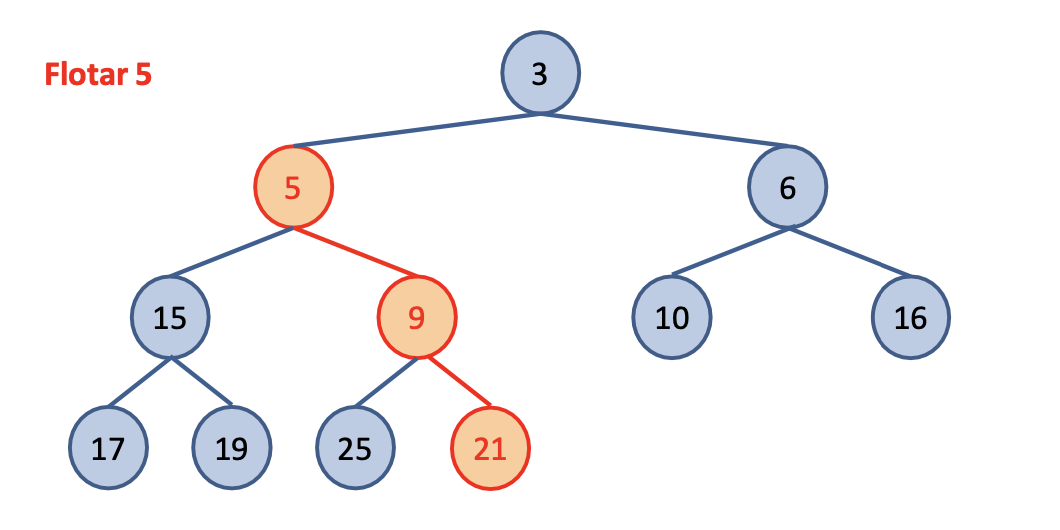
\includegraphics[width=0.7\textwidth]{assets/apo3.png}
  \end{center}
  \caption{Ejemplo de inserción 2.}
\end{figure}
Tenemos como resultado que el nodo con valor `5' es el nuevo hijo izquierdo del nodo raíz, y por tanto, vemos que todos los nodos están ordenados.
\subsubsection*{Código de Inserción y Flotar}

\underbar{Código de insertar:}
\begin{minted}[breaklines]{C++}
template <typename T> void Apo<T>::insertar(const T& e){
  assert(numNodos < maxNodos);
  //insertamos en la última posición.
  nodos[numNodos] = e; 
  //Llamamos al método flotar
  if(numNodos > 1)
    flotar(numNodos-1);
}
  \end{minted}
\underbar{Código de flotar:}
\begin{minted}[breaklines]{C++}
template <typename T> void Apo<T>::flotar(nodo n){
  //Guardamos el contenido del nodo
  T e = nodos[n];
  //recorremos los nodos intercambiandolos
  while(n>0 && e < nodos[padre(n)]){
    nodos[n] = nodos[padre(n)];
    n = padre(n);
  }
  nodos[n] = e;
}
\end{minted}

\subsection*{Eliminación de elementos en un APO}
\begin{figure}[h]
  \begin{center}
    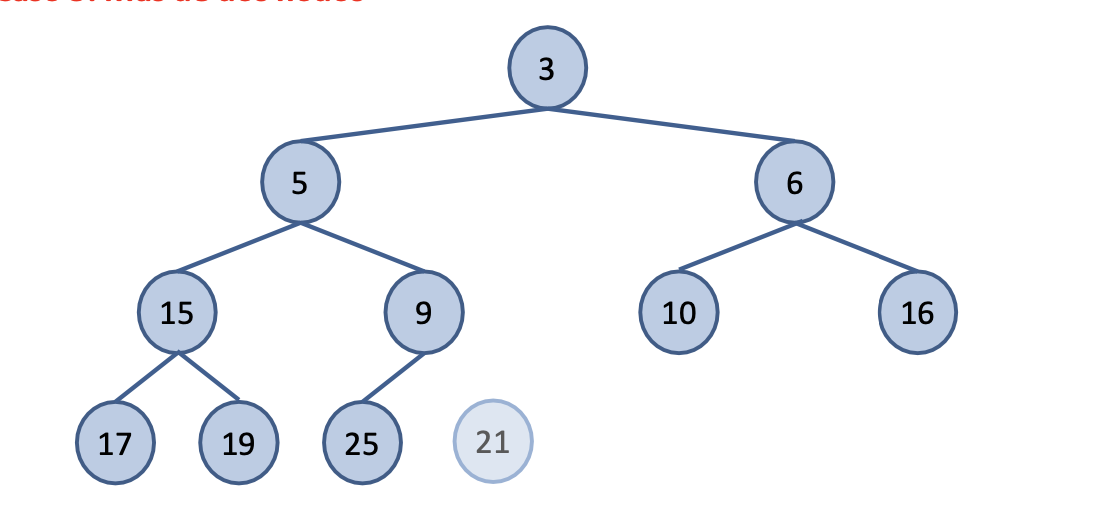
\includegraphics[width=0.7\textwidth]{assets/apo4.png}
  \end{center}
\end{figure}

Vemos que queremos realizar la eliminación del nodo raíz con contenido `3', por tanto, el último nodo del árbol `21', ocupará la posición del nodo raíz sobrescribiendo su contenido y por ende tendremos que hundir dicho nodo para que el APO siga ordenado.
\begin{figure}[h]
  \begin{center}
    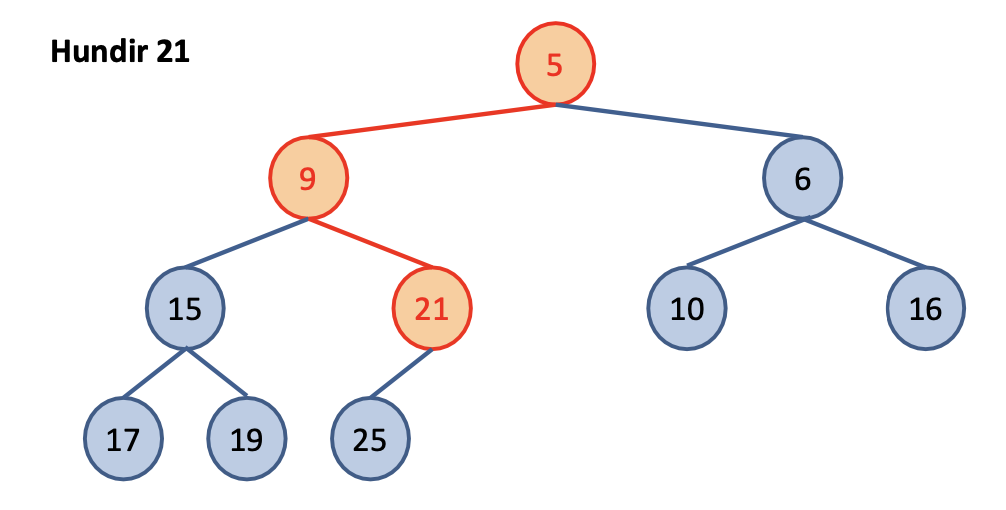
\includegraphics[width=0.7\textwidth]{assets/apo5.png}
  \end{center}
\end{figure}

COmo resultado tenemos que el nodo con valor `21' ahora es padre del nodo con valor `25' y el nuevo nodo raíz es el nodo con valor `5' que previamente era el hijo izquierdo del nodo con valor `3' (la raíz anterior).

\underbar{Código de suprimir:}
\begin{minted}[breaklines]{C++}
template <typename T> void Apo<T>::suprimir(){
  assert(numNodos > 0);
  if(--numNodos > 0){
    nodos[0]=nodos[numNodos];
    if(numNodos > 1)
      hundir(0);
  }
}
\end{minted}
\underbar{Código de hundir:}\\
\begin{minted}[breaklines]{C++}
template <typename T> void Apo<T>::hundir(nodo n){
  bool fin = false;
  T e = nodos[i];
  while (hIzq(i) < numNodos && !fin){
    nodo hMin;
    if (hDer(i) < numNodos && nodos[hDer(i)] 
        < nodos[hIzq(i)])
    hMin = hDer(i);
    else
      hMin = hIzq(i);
      if (nodos[hMin] < e){
        nodos[i] = nodos[hMin];
        i = hMin;
      }
    else
      fin = true;
  }
  nodos[i] = e;
}
\end{minted}

Finalmente, como conclusión sacamos de que un \textbf{APO} no es un \textbf{AVL}, ya que ambos tienen propositos diferentes, siendo el objetivo principal de los AVLs la búsqueda de elementos lo más rapido posible y en los APOs su uso en algoritmos de ordenación y en el uso de colas con prioridad.
